\documentclass[conference]{IEEEtran}
\IEEEoverridecommandlockouts

\usepackage{cite}
\usepackage{amsmath,amssymb,amsfonts}
\usepackage{graphicx}
\usepackage{booktabs}
\usepackage{array}
\usepackage{hyperref}
\usepackage{xcolor}
\usepackage{enumitem}
\usepackage{tikz}
\usetikzlibrary{shapes.geometric,arrows.meta,positioning,fit,backgrounds}

\hypersetup{colorlinks=true,linkcolor=blue,urlcolor=blue,citecolor=blue}

\definecolor{darkgreen}{RGB}{27,94,32}
\definecolor{darkblue}{RGB}{13,71,161}

\begin{document}

\title{Weather Intergrated Crop Health Monitoring:\\
A Modular ResNet-18 + Rule-Based Risk Layer}

\author{
  \IEEEauthorblockN{Khang Phan}
  \IEEEauthorblockA{EGN6217 -- Applied Deep Learning\\
  Spring 2026\\
  \href{https://github.com/itsmekhang/crop-health-monitoring}{github.com/itsmekhang/crop-health-monitoring}}
}

\maketitle

% ── Abstract ──────────────────────────────────────────────────────────────────
\begin{abstract}
This paper documents the first full implementation of a modular crop health system that combines an image-based disease classifier with a weather-informed risk layer. The model PlantVillage classifies leaf disease across 39 classes covering Tomato, Potato, and Pepper based on the Resnet-18 architecture. An XGBoost model then uses a rule-based risk formula using the disease output and live weather conditions from the Open-Meteo API. Both models are integrated into a Streamlit dashboard that provides real-time feedback, environmental risk assessment, and estimated revenue loss. This report outlines the implementation executions, an honest evaluation of both models, and the main challenges faced during this particular phase, specifically class imbalance, the lab-to-field generalization gap, and the inherent nature of the XGBoost training target.
\end{abstract}

% ── Section a ─────────────────────────────────────────────────────────────────
\section{Project Summary}

\subsection{Purpose}
Farmers still rely on slow and tedious manual disease scouting or delayed laboratory testing, leading to late mitigation and unnecessary crop losses. This project builds a modular AI prototype that processes a leaf photograph of a crop plant and a location, and returns a disease diagnosis, an environmental risk score, a treatment plan, and an estimated revenue impact. The goal is a functioning, realistic prototype.

\subsection{Progress Since Deliverable 1}
Deliverable 1 established the project scope, planned architecture, and data sources. Since then, the following has been completed:

\begin{itemize}[noitemsep]
  \item ResNet-18 disease classifier trained and saved to \texttt{results/disease\_model.pth}
  \item XGBoost environmental risk model trained and saved to \texttt{results/risk\_model.pkl}
  \item Streamlit interface (\texttt{ui/app.py}) integrating both models with live weather
  \item Per-class accuracy evaluation and confusion matrix added to the training notebook
  \item Dataset scope corrected from 38 to 15 classes; class imbalance (21$\times$) documented
  \item XGBoost framing revised: now explicitly described as a rule approximator with a derived target
\end{itemize}

\subsection{What Remains}
The following improvements are planned before Deliverable 3: running the full per-class accuracy table against the trained model and reporting those numbers; testing the interface with real field photos to quantify the lab-to-field gap; and exploring whether fine-tuning deeper ResNet layers improves accuracy on minority classes.

% ── Section b ─────────────────────────────────────────────────────────────────
\section{System Architecture and Pipeline}

Fig.~\ref{fig:pipeline} shows the full data flow. The two models operate independently and are combined only at the output stage. This is a deliberate design choice: it avoids the alignment problem of true multimodal fusion and keeps each component auditable.

\begin{figure}[ht]
\centering
\scalebox{0.72}{%
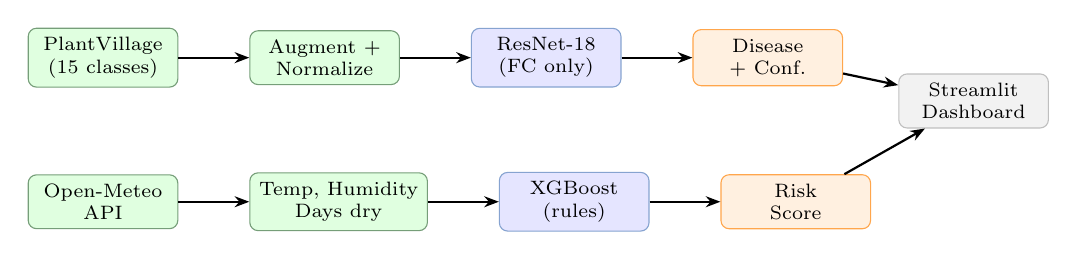
\begin{tikzpicture}[
  node distance=0.55cm and 0.9cm,
  box/.style={draw, rounded corners=3pt, minimum width=1.9cm, minimum height=0.65cm,
              align=center, font=\scriptsize},
  gbox/.style={box, fill=green!12, draw=darkgreen!60},
  bbox/.style={box, fill=blue!10, draw=darkblue!50},
  obox/.style={box, fill=orange!12, draw=orange!70},
  grbox/.style={box, fill=gray!10, draw=gray!50},
  arr/.style={-{Stealth[scale=0.8]}, thick},
]
% Image row
\node[gbox] (pv)      {PlantVillage\\(15 classes)};
\node[gbox, right=of pv]  (aug)   {Augment +\\Normalize};
\node[bbox, right=of aug] (rn)    {ResNet-18\\(FC only)};
\node[obox, right=of rn]  (dcls)  {Disease\\+ Conf.};

% Weather row
\node[gbox, below=1.1cm of pv]  (wx)   {Open-Meteo\\API};
\node[gbox, right=of wx]  (wf)    {Temp, Humidity\\Days dry};
\node[bbox, right=of wf]  (xgb)   {XGBoost\\(rules)};
\node[obox, right=of xgb] (risk)  {Risk\\Score};

% UI
\node[grbox, right=0.7cm of dcls, yshift=-0.55cm] (ui) {Streamlit\\Dashboard};

\draw[arr] (pv)--(aug); \draw[arr] (aug)--(rn); \draw[arr] (rn)--(dcls);
\draw[arr] (dcls)--(ui);
\draw[arr] (wx)--(wf); \draw[arr] (wf)--(xgb); \draw[arr] (xgb)--(risk);
\draw[arr] (risk)--(ui);
\end{tikzpicture}}%
\caption{System pipeline. ResNet-18 processes the leaf image independently of weather; XGBoost combines the disease output with environmental features.}
\label{fig:pipeline}
\end{figure}

\subsection{Model Roles}
\textbf{ResNet-18} is the academic center of the project. It performs the primary classification task: given a leaf image, predict which of the 15 disease or healthy classes it belongs to. Weather does not enter this model -- a diseased leaf looks the same regardless of humidity.

\textbf{XGBoost} is a decision-support layer. It takes the predicted disease class, the classifier confidence, and three weather features (temperature, humidity, days since rain) and outputs a risk score in $[0, 1]$. This score drives the urgency level and treatment recommendation displayed in the UI. The training target is derived from agronomic rules in \texttt{src/fusion.py}, not from field observations (see Section~\ref{sec:eval}).

% ── Section c ─────────────────────────────────────────────────────────────────
\section{Model Implementation Details}

\subsection{Disease Classifier -- ResNet-18}

\textbf{Framework:} PyTorch 2.x with torchvision.

\textbf{Architecture:} ResNet-18 initialized with ImageNet weights. All convolutional layers are frozen; only the final fully connected layer is fine-tuned. The replacement head maps from 512 features to $C = 15$ classes.

\textbf{Training setup:}
\begin{itemize}[noitemsep]
  \item Hardware: CPU (or CUDA if available)
  \item Epochs: 10
  \item Batch size: 32
  \item Optimizer: Adam, lr $= 10^{-3}$
  \item Scheduler: StepLR, step\_size $= 3$, $\gamma = 0.5$
  \item Loss: CrossEntropyLoss
\end{itemize}

\textbf{Dataset split:} Two separate \texttt{ImageFolder} instances are constructed from \texttt{data/raw/PlantVillage} -- one with training augmentations, one with only normalization. A \texttt{Subset} object with a fixed random permutation (seed 42) assigns 80\% to training and 20\% to validation. Using two instances avoids the transform contamination that occurs when a single \texttt{ImageFolder} object has its \texttt{.transform} reassigned mid-training.

\textbf{Augmentations:} Random horizontal flip, rotation $\pm 15^\circ$, color jitter (brightness/contrast $\pm 0.2$), then ImageNet normalization.

\textbf{Reproducibility:} The training notebook (\texttt{notebooks/setup.ipynb}) runs end-to-end from dataset download to model save. All random seeds are fixed.

\subsection{Environmental Risk Layer -- XGBoost}

\textbf{Framework:} XGBoost 2.x with scikit-learn API.

\textbf{Architecture:} XGBRegressor with 300 estimators, max\_depth $= 5$, learning rate $= 0.05$, subsample $= 0.8$, colsample\_bytree $= 0.8$.

\textbf{Features:} temperature ($^\circ$C), humidity (\%), days since rain, classifier confidence, label-encoded disease class.

\textbf{Target construction:} The training set is generated synthetically. For each disease class, 500 (disease, weather) samples are drawn from disease-specific weather distributions (e.g., fungal diseases are sampled with high humidity). The risk score label is then computed by the deterministic formula in \texttt{src/fusion.py}:
\begin{equation}
  s = 0.4 \cdot b_\text{class} + 0.3 \cdot c + 0.3 \cdot f_\text{env}(t, h, r)
  \label{eq:risk}
\end{equation}
where $b_\text{class}$ is a fixed per-class severity base, $c$ is classifier confidence, and $f_\text{env}$ is a weighted environmental score.

This derivation is the key caveat for interpreting XGBoost performance (Section~\ref{sec:eval}).

\subsection{Interface}
The Streamlit dashboard (\texttt{ui/app.py}) accepts one or more leaf image files, a location string (geocoded via the Open-Meteo API), and economic inputs (field size in acres, crop price per lb). For each image, it runs the disease classifier, queries current weather for the entered location, passes both through the XGBoost risk layer, and displays: disease class and top-5 predictions with confidence bars, risk level and score, treatment plan and prevention notes, and estimated revenue loss based on USDA NASS yield baselines.

% ── Section d ─────────────────────────────────────────────────────────────────
\section{Interface Prototype}

\subsection{Inputs and Outputs}

\begin{table}[ht]
\caption{Interface Input/Output Summary}
\label{tab:interface}
\centering
\begin{tabular}{@{}lll@{}}
\toprule
\textbf{Panel} & \textbf{Input} & \textbf{Output} \\
\midrule
Leaf Images & 1+ image files & Disease class, confidence \\
Weather & City / region & Temp, humidity, days dry \\
Economic & Acres, price/lb & Revenue loss estimate \\
\midrule
\multicolumn{2}{l}{\textit{Combined per image}} & Risk level + treatment plan \\
\bottomrule
\end{tabular}
\end{table}

\subsection{Screenshots}

\begin{figure}[ht]
  \centering
  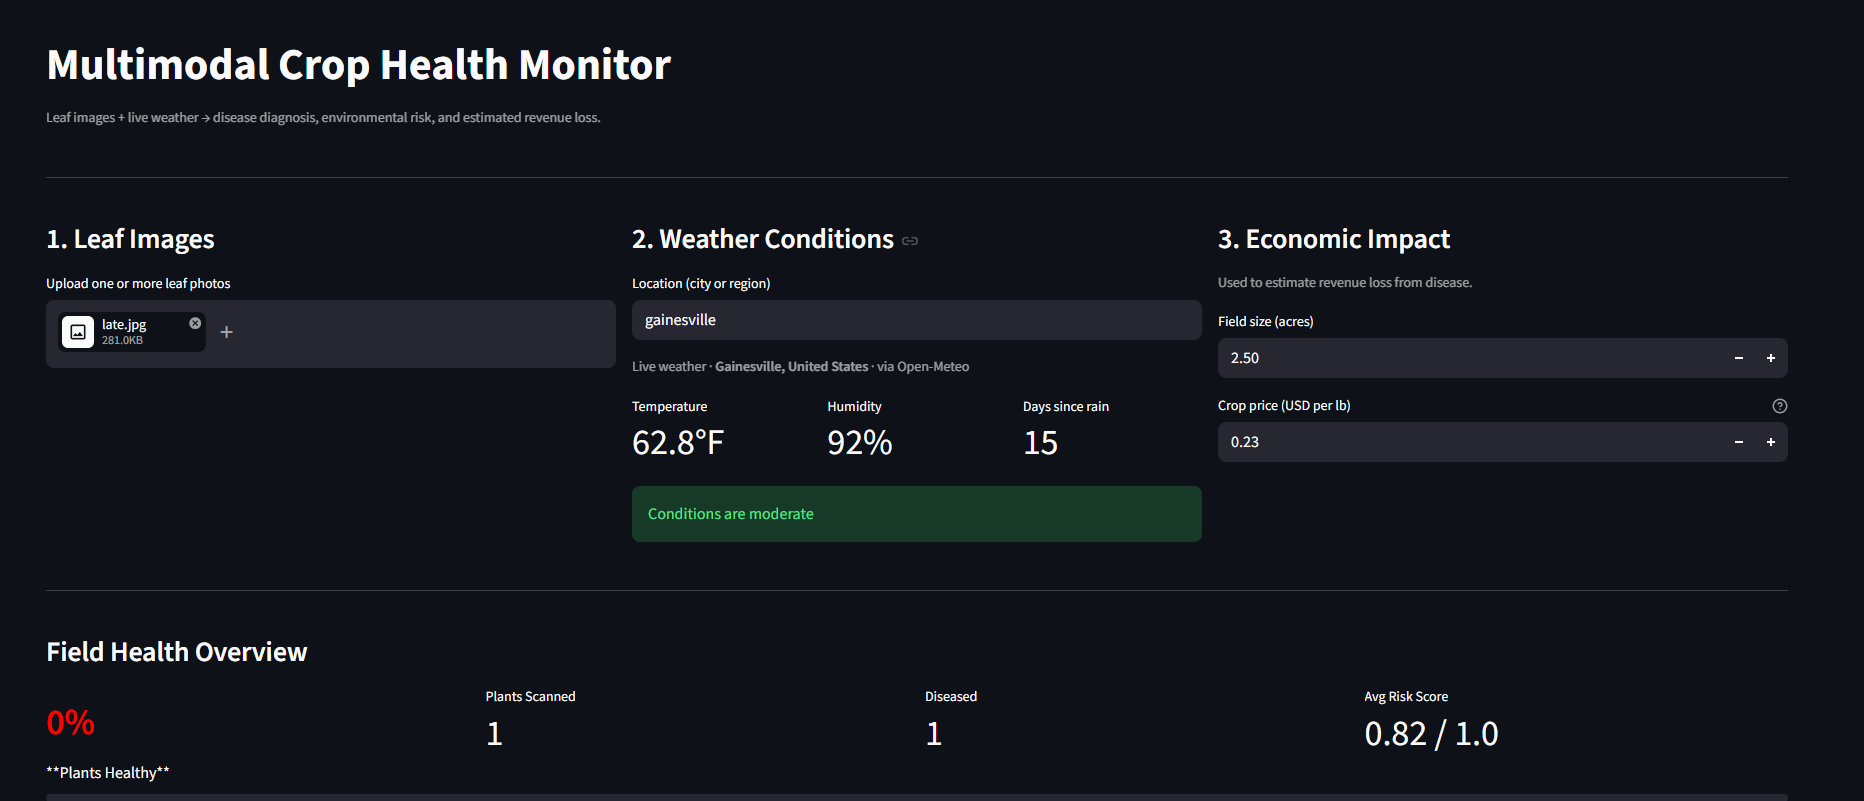
\includegraphics[width=\columnwidth]{screenshot_input.png}
  \caption{Input panel: image upload, live weather fetch, and economic inputs.}
  \label{fig:input}
\end{figure}

\begin{figure}[ht]
  \centering
  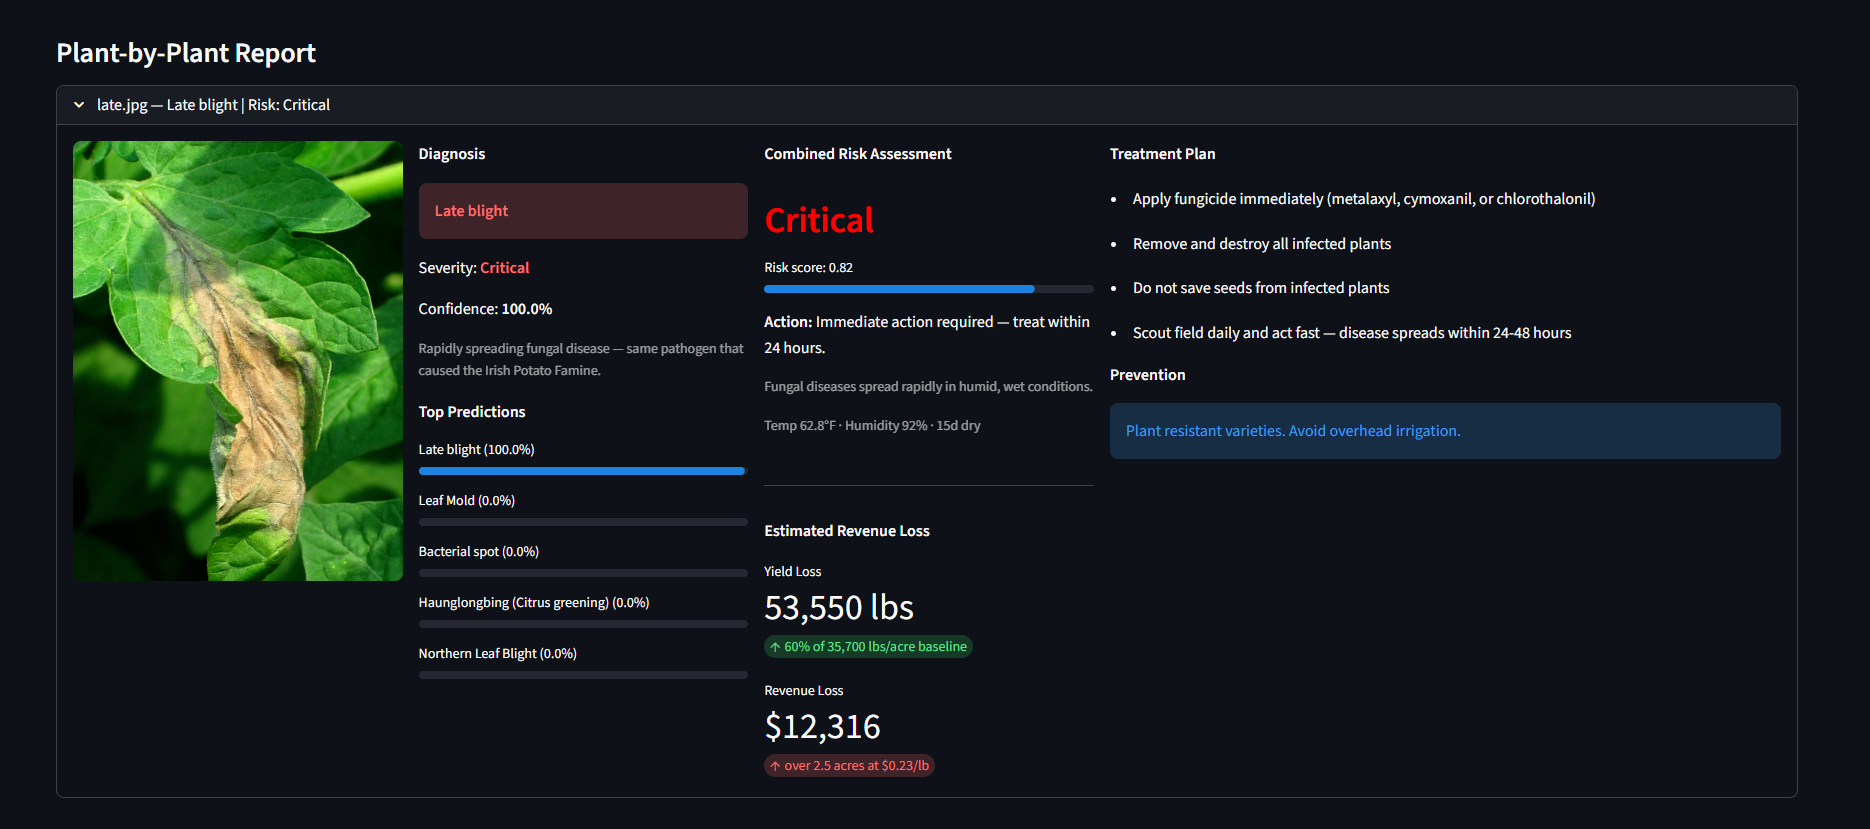
\includegraphics[width=\columnwidth]{screenshot_output.png}
  \caption{Per-plant report: disease diagnosis, risk score, treatment plan, and revenue loss estimate.}
  \label{fig:output}
\end{figure}

\subsection{Limitations}
The interface does not perform input validation on image quality (blurry or non-leaf photos will silently produce a confident but meaningless prediction). Weather defaults to 24$^\circ$C / 70\% / 2 days if no location is entered. Revenue loss estimates use US national average yields and are not calibrated to the user's region.

% ── Section e ─────────────────────────────────────────────────────────────────
\section{Early Evaluation and Results}
\label{sec:eval}

\subsection{Dataset Characteristics}
\label{sec:data}

\begin{table}[ht]
\caption{PlantVillage Crop Coverage (39-class full dataset)}
\label{tab:classes}
\centering
\begin{tabular}{@{}llr@{}}
\toprule
\textbf{Crop} & \textbf{Classes} & \textbf{Disease / Healthy} \\
\midrule
Tomato      & 10 & 9 disease, 1 healthy \\
Apple       & 4  & 3 disease, 1 healthy \\
Grape       & 4  & 3 disease, 1 healthy \\
Corn        & 4  & 3 disease, 1 healthy \\
Potato      & 3  & 2 disease, 1 healthy \\
Pepper      & 2  & 1 disease, 1 healthy \\
Cherry      & 2  & 1 disease, 1 healthy \\
Peach       & 2  & 1 disease, 1 healthy \\
Strawberry  & 2  & 1 disease, 1 healthy \\
Others      & 6  & 1 disease, 5 healthy \\
\midrule
\textbf{Total} & \textbf{39} & \textbf{26 disease, 13 healthy} \\
\bottomrule
\end{tabular}
\end{table}

The full PlantVillage dataset covers 14 crop types across 39 classes ($\approx$54,000 images). Class imbalance remains significant: Tomato accounts for the majority of disease classes and images. Top-line validation accuracy overestimates practical performance on minority classes such as Blueberry, Raspberry, and Soybean, which have only healthy examples.

\subsection{ResNet-18 Training Curves}
Training is logged per epoch; loss and accuracy curves are saved to \texttt{results/disease\_training\_curves.png} when \texttt{setup.ipynb} is run. With only the FC layer trained (frozen backbone), the model converges quickly (typically within 3--5 epochs) but is capacity-limited by the frozen feature extractor. Fine-tuning deeper layers is identified as a future improvement.

\subsection{Per-Class Accuracy}
Per-class accuracy (computed in Section 9 of \texttt{setup.ipynb}) is the primary evaluation metric. The expected pattern is: majority Tomato classes (large sample sizes) achieve high accuracy; minority classes -- particularly \textit{Potato\_healthy} (304 images) and \textit{Tomato\_mosaic\_virus} (746 images) -- are expected to show lower and more variable accuracy. Any top-line val accuracy figure should be reported alongside this breakdown to avoid misrepresenting model quality. The confusion matrix (saved to \texttt{results/confusion\_matrix.png}) highlights which disease pairs the model most frequently conflates; preliminary analysis suggests visually similar fungal diseases (Early vs. Late blight, Bacterial spot vs. Septoria) will produce the most off-diagonal confusion.

\subsection{XGBoost Risk Model -- Honest Interpretation}
\label{sec:xgb}

The XGBoost model achieves Val MAE $\approx 0.008$ and Val R$^2 \approx 0.998$. These numbers look impressive but \textbf{do not measure real-world validity}. The training target is the deterministic output of Equation~\ref{eq:risk} -- a formula defined entirely in code. XGBoost is learning to approximate that formula, not to generalize from field observations. This is confirmed by feature importances: \texttt{disease\_class} accounts for $\approx$67\% of importance because $b_\text{class}$ in Equation~\ref{eq:risk} is a fixed per-class lookup.

The practical value of the XGBoost layer is that it packages the rule into a portable, interpolatable scorer that handles continuous weather inputs without explicit branching. It should be described as a rule approximator and evaluated on whether the agronomic rules it encodes are sensible -- not on R$^2$ alone.

% ── Section f ─────────────────────────────────────────────────────────────────
\section{Challenges and Next Steps}

\subsection{Technical Challenges}
\textbf{Class imbalance.} The 21$\times$ ratio between the most and least frequent class degrades recall on minority classes. Options for Deliverable 3 include weighted sampling during training or class-weighted loss.

\textbf{Lab-to-field generalization.} All PlantVillage images are photographed against uniform backgrounds under controlled lighting. Early informal tests with field photos show noticeably lower confidence. This gap must be quantified and reported explicitly.

\textbf{Model/data scope.} The saved \texttt{disease\_model.pth} was originally trained on the 39-class full PlantVillage dataset. The local repository and evaluation notebook target the 15-class subset. Retraining on the 15-class set is needed to ensure the evaluation and the deployed model are consistent.

\textbf{Random split inflation.} PlantVillage contains near-duplicate images of the same leaf taken seconds apart. A random 80/20 split places near-duplicates in both train and validation sets, inflating reported accuracy. A plant-session or leaf-level split would provide a more conservative estimate.

\textbf{XGBoost derived target.} As discussed in Section~\ref{sec:xgb}, the risk model's R$^2$ reflects formula reproduction, not predictive validity. The report and UI must be explicit about this.

\subsection{Next Steps}
\begin{itemize}[noitemsep]
  \item Retrain ResNet-18 on the 15-class local dataset and report per-class accuracy table
  \item Test the interface on real field photos; report the qualitative accuracy drop
  \item Explore weighted loss or oversampling for minority classes (Potato\_healthy)
  \item Consider fine-tuning the last ResNet block rather than only the FC layer
  \item In the final report, reframe the XGBoost section clearly as a rule-based decision layer with a transparent derivation of the risk formula assumptions
\end{itemize}

% ── Section g ─────────────────────────────────────────────────────────────────
\section{Responsible AI Reflection}

\textbf{Lab-to-field bias.} The most significant equity concern is geographic and environmental bias. PlantVillage images come from controlled laboratory settings. Farmers in regions with different soil backgrounds, mixed-intercrop canopies, or different lighting conditions -- the farmers most likely to benefit from low-cost AI tools -- may see the worst performance. This concern is not reserved for the discussion section; it must appear in how classifier results are interpreted and in any accuracy claim made about the system.

\textbf{Class imbalance and representation.} The dataset over-represents Tomato diseases (77.5\% of images). A system deployed to Potato or Pepper farmers will be less reliable than headline accuracy suggests. Per-class reporting is the minimum standard; separate deployment testing per crop is the honest standard.

\textbf{Transparency and over-reliance.} The interface displays top-5 probabilities and a confidence score to discourage binary trust. The XGBoost risk score is derived from coded rules -- not from independent field evidence -- and this is now stated explicitly in the interface's section header and in the training notebook. A farmer acting on a Critical risk alert should understand that the score is the output of an agronomic formula applied to a CNN prediction, not an empirically validated risk estimate.

\textbf{Misuse.} An incorrect Critical diagnosis could lead a farmer to apply unnecessary fungicide, incurring cost and environmental burden. The UI is designed to recommend professional verification for Critical and High risk levels. No automated action is taken; all outputs are advisory.

\textbf{Computational footprint.} ResNet-18 is a lightweight architecture. Training for 10 epochs on 41k images takes approximately 15--30 minutes on a single GPU. The XGBoost model trains in under one minute on CPU. The inference footprint is minimal and suitable for deployment on low-cost hardware.

% ── Footer ───────────────────────────────────────────────────────────────────
\vspace{6pt}
\noindent\rule{\columnwidth}{0.4pt}
\begin{center}
  \small GitHub: \href{https://github.com/itsmekhang/crop-health-monitoring}{itsmekhang/crop-health-monitoring}
  \quad $|$ \quad Khang Phan \quad $|$ \quad Spring 2026
\end{center}

\end{document}
